\subsection{Quantitative data}

    %What the data said

    \subsubsection{Results from the coaches}

    \subsubsection{Day 2}
    Most coaches prefer tablet: 5 prefer tablet, 2 smartphone, and 2 computer.

    \subsubsection{Day 3}
    iOS no longer allows uncertified app install from computer: you need to have paid a license even for unreleased apps, being a "Trusted developer". This stops the app from being able to be installed on all the iOS devices, so that only the web version can be used.

    Thus, only the web app was tested from Wednesday and onwards.

    This was a problems, as the app regurly crashed at refresh because of low internet capacity.

    Sometimes, it was neeed to go to the other office where there was wifi, to refresh the webpage, and go back to the location. This of course would not work for Josefina.

    \subsubsection{Day 4}
    Tested using the quiz before the session.  Using the quiz before the session increases learning, slightly decreases fun of the session, according to coaches. It is "Fun and encouraging".

    \subsubsection{Day 5}
    On day 5, the schedule was:

    \begin{itemize}
      \item "Goal setting" part 2
      \item App test: "Goal setting" after-quiz and "Graduation" pre-quiz.
      \item "Graduation"
    \end{itemize}

    In "Goal setting", one coach were an outlier to the other high results, scoring 9/19 answers correct.

    \subsubsection{Results from workshop \#2}

    During this workshop, the focus was to examine what builds confidence among the coaches. The following clusters could be determined: "I believe in myself" (3 coaches), "I believe in God" (2 coaches), "I am well prepared" (4 coaches) and "I am certified" (1 coach). See figure \ref{fig:zambiaWorkshop2} for the different clusters.

    \begin{figure}[h]
        \centering
        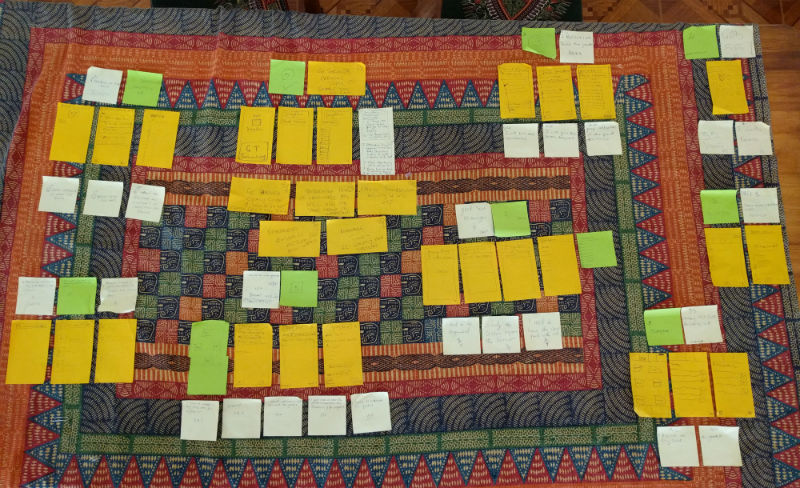
\includegraphics[width=0.7\textwidth]{zambiaWorkshop2small.jpg}
        \caption{The clustered postits with needs, together with included design proposals.}
        \label{fig:iteration}
    \end{figure}

    \subsubsection{Bonus results: Testing the app on refugee innovations}
    Back in Uganda, a test was done with refugee innovators, at the Humanitarian Innovation Jam.

    The test with the refugee innovatiors were surprisingly intriguing and successful.

    It was found that refugee innovators says they would have a great need for such an app.
